\documentclass[a4paper]{article}
\usepackage{amsmath}
\usepackage{amsfonts,amssymb}
\usepackage[utf8]{inputenc}
\usepackage[colorlinks,citecolor=blue,urlcolor=blue]{hyperref}
\usepackage{graphicx,xcolor}
\usepackage{tikz}
\usetikzlibrary{arrows.meta, positioning}

\begin{document}

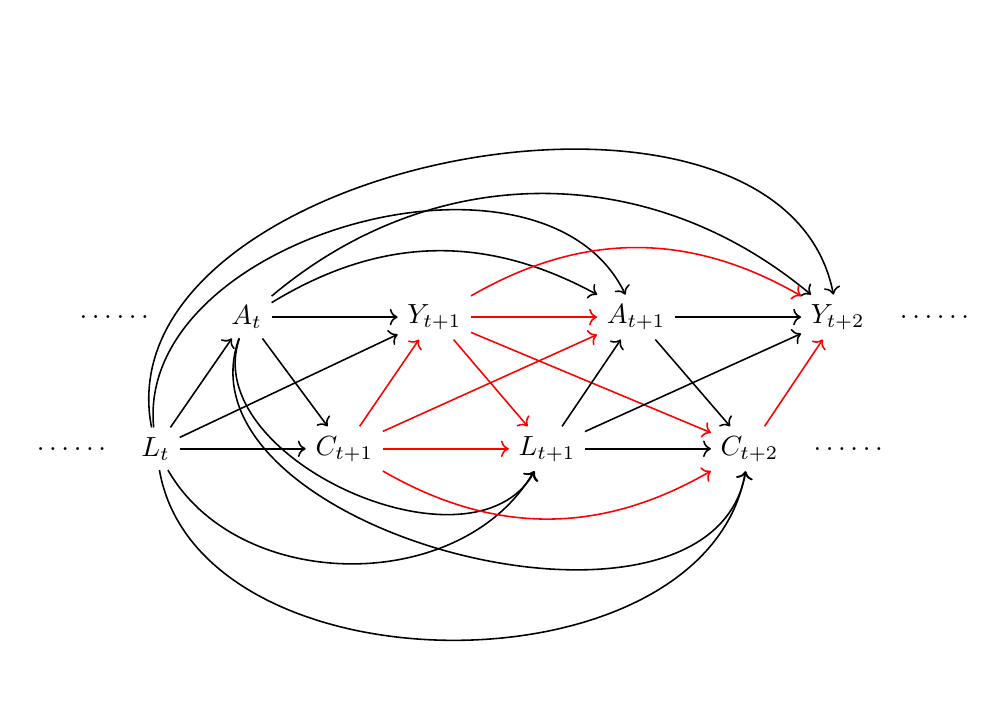
\begin{tikzpicture}[node distance=1.6cm, auto]
	% Nodes
	\node (Lt) {$L_t$};
	\node[right=of Lt] (Ct1) {$C_{t+1}$};
	\node[right=of Ct1] (Lt1) {$L_{t+1}$};
	\node[right=of Lt1] (Ct2) {$C_{t+2}$};
	\node[above right=of Lt, xshift=-0.6cm] (At) {$A_t$};
	\node[right=of At] (Yt1) {$Y_{t+1}$};
	\node[right=of Yt1] (At1) {$A_{t+1}$};
	\node[right=of At1] (Yt2) {$Y_{t+2}$};
	\node[left=of Lt, xshift=1.4cm] (ldot1) {$\ldots\ldots$};
	\node[left=of At, xshift=0.8cm] (ldot2) {$\ldots\ldots$};
	\node[right=of Ct2, xshift=-1.4cm] (ldot3) {$\ldots\ldots$};
	\node[right=of Yt2, xshift=-1.4cm] (ldot4) {$\ldots\ldots$};

	% Edges
	\draw[->, black, line width=0.2mm] (Lt) -- (At);
	\draw[->, black, line width=0.2mm] (Lt) -- (Ct1);
	\draw[->,black, line width=0.2mm] (Lt) -- (Yt1);
	\draw[->, black, line width=0.2mm] (At) -- (Yt1);
	\draw[->, black, line width=0.2mm] (At) -- (Ct1);
	\draw[->, red, line width=0.2mm] (Ct1) -- (Yt1);
	\draw[->, red, line width=0.2mm] (Yt1) -- (At1);
	\draw[->, red, line width=0.2mm] (Yt1) -- (Lt1);
	\draw[->, red, line width=0.2mm] (Yt1) -- (Ct2);
	\draw[->, red, line width=0.2mm] (Ct1) -- (Lt1);
	\draw[->, red, line width=0.2mm] (Ct1) -- (At1);
	\draw[->,black, line width=0.2mm] (Lt1) -- (At1);
	\draw[->,black, line width=0.2mm] (At1) -- (Yt2);
	\draw[->,black, line width=0.2mm] (At1) -- (Ct2);
	\draw[->,black, line width=0.2mm] (Lt1) -- (Ct2);
	\draw[->,black, line width=0.2mm] (Lt1) -- (Yt2);
	\draw[->,red, line width=0.2mm] (Ct2) -- (Yt2);

	% Bend
	% Lt
	\draw[->, bend left=80,black, line width=0.2mm] (Lt) to (At1);
	\draw[->, bend left=90,black, line width=0.2mm] (Lt) to (Yt2);
	\draw[->, bend right=60,black, line width=0.2mm] (Lt) to (Lt1);
	\draw[->, bend right=80,black, line width=0.2mm] (Lt) to (Ct2);
	% At
	\draw[->, bend left=30,black, line width=0.2mm] (At) to (At1);
	\draw[->, bend left=40,black, line width=0.2mm] (At) to (Yt2);
	\draw[->, bend right=85,black, line width=0.2mm] (At) to (Lt1);
	\draw[->, bend right=95,black, line width=0.2mm] (At) to (Ct2);
	% Yt1
	\draw[->, bend left=30,red, line width=0.2mm] (Yt1) to (Yt2);
	% Ct1
	\draw[->, bend right=30,red, line width=0.2mm] (Ct1) to (Ct2);

\end{tikzpicture}

\end{document}